\section{2d Web Symbols and Icons}


\begin{figure}
	\centering
	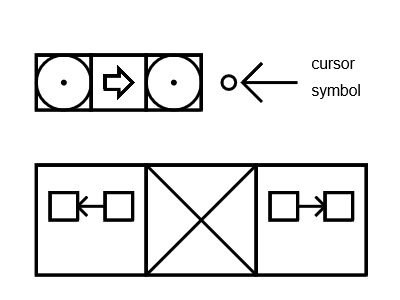
\includegraphics[width=3in]{figures/web2d/cursoredit.png}
	\caption[cursoredit]
	{cursor edits.}
\end{figure}

\begin{figure}
	\centering
	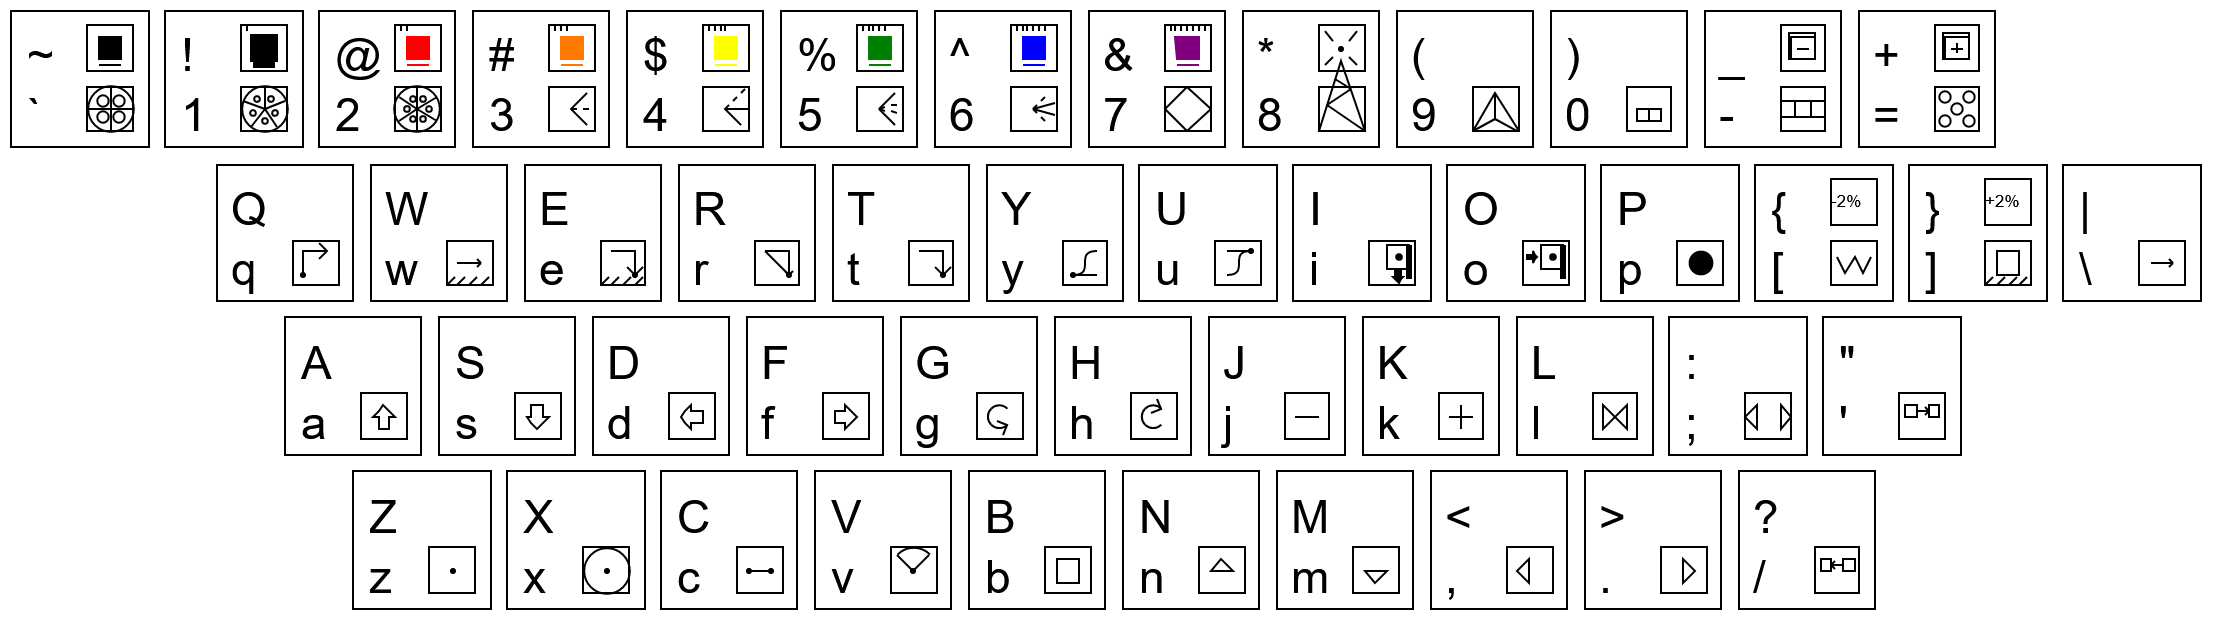
\includegraphics[width=4in]{figures/web2d/keyboard.png}
	\caption[keyboard]
	{keyboard.}
\end{figure}

\begin{figure}
	\centering
	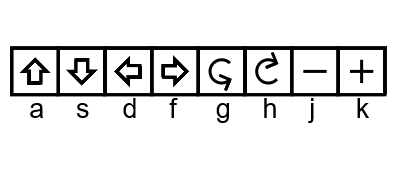
\includegraphics[width=4in]{figures/web2d/move.png}
	\caption[move]
	{Movements.  Arrows move along directions of the lines in the cursor.  Rotation is by the unit indicated by the cursor wing angles. Scale actions are by the current scale value as shown by the dot positions on the cursor.  Letters shown indicate the keys which map to these actions on a QWERTY keyboard with the default settings.}
\end{figure}

\begin{figure}
	\centering
	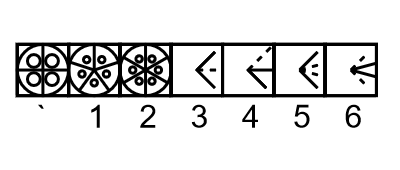
\includegraphics[width=4in]{figures/web2d/angles.png}
	\caption[angles]
	{Angles described by symmetry glyphs.  This also shows the actions to bisect, double, trisect and triple angles, and what keys are used to activate each geometric action.}
\end{figure}

\begin{figure}
	\centering
	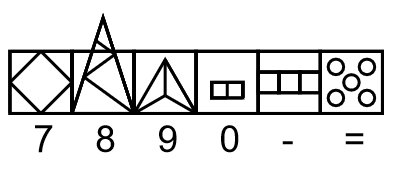
\includegraphics[width=4in]{figures/web2d/scaleactions.png}
	\caption[scaleactions]
	{Scales, along with keys used to map to them in default configuration. There is no relation between the numbers on the keys and the mathematics of the scales.  The scales shown are, from left to right, the square root of 2, the Golden Ratio, the square root of 3, 2, 3, and 5.}
\end{figure}

\begin{figure}
	\centering
	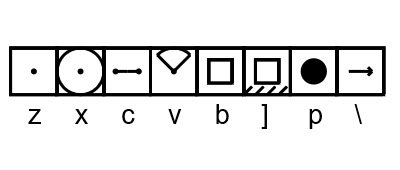
\includegraphics[width=4in]{figures/web2d/basicdraw.png}
	\caption[basicdraw]
	{Basic drawing actions, along with keys used in default configuration to activate them.  From left to right the actions are: draw dot, draw circle of unit radius, draw line segment of unit length, draw arc between cursor wings, draw a square, draw a filled square, draw a filled circle, and draw a line segment while moving forward one unit.}
\end{figure}

\begin{figure}
	\centering
	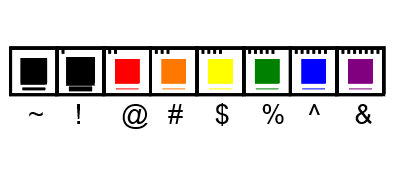
\includegraphics[width=4in]{figures/web2d/colors.png}
	\caption[colors]
	{Layers. Each layer has a line color, line width, and fill color, all of which are set with the Style object using the Style editor app.}
\end{figure}

\begin{figure}
	\centering
	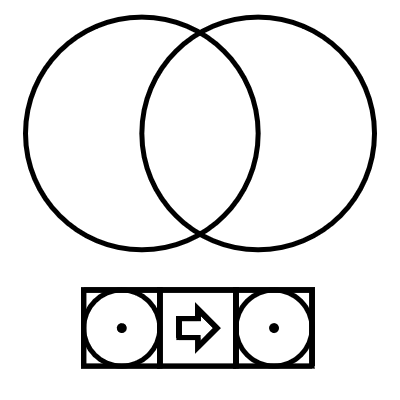
\includegraphics[width=4in]{figures/web2d/vesicapiscis.png}
	\caption[vesicapiscis]
	{The ``hello world'' of geometric programming, the Vesica Piscis.}
\end{figure}
\begin{figure}
	\centering
	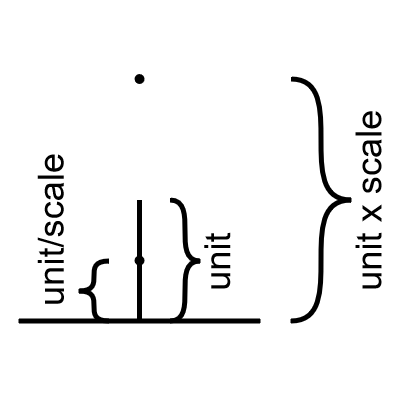
\includegraphics[width=4in]{figures/web2d/cursorscale1.png}
	\caption[cursorscale]
	{Cursor scale.}
\end{figure}
\begin{figure}
	\centering
	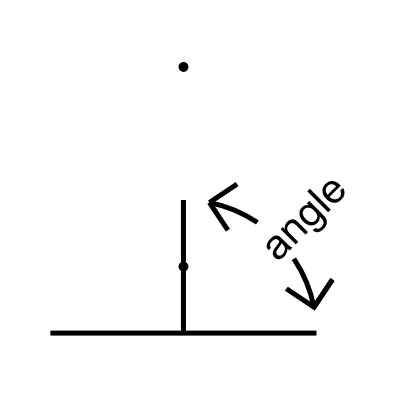
\includegraphics[width=4in]{figures/web2d/cursorangle1.png}
	\caption[cursorangle]
	{Cursor angle.}
\end{figure}
\begin{figure}
	\centering
	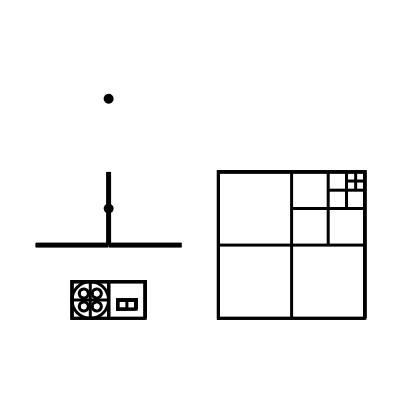
\includegraphics[width=4in]{figures/web2d/cursorsquare.png}
	\caption[cursorsquare]
	{Cursor square.}
\end{figure}
\begin{figure}
	\centering
	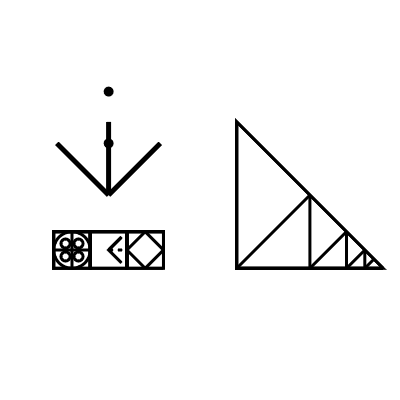
\includegraphics[width=4in]{figures/web2d/cursorroot2.png}
	\caption[cursorroot2]
	{Cursor root2.}
\end{figure}
\begin{figure}
	\centering
	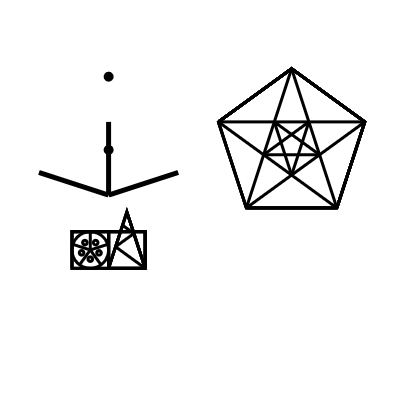
\includegraphics[width=4in]{figures/web2d/cursorgolden.png}
	\caption[cursorgolden]
	{Cursor golden ratio.}
\end{figure}
\begin{figure}
	\centering
	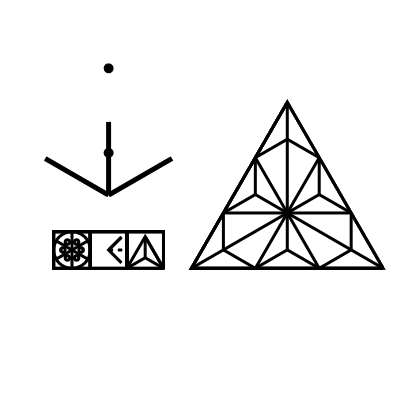
\includegraphics[width=4in]{figures/web2d/cursorroot3.png}
	\caption[cursorroot3]
	{Cursor root 3.}
\end{figure}
\begin{figure}
	\centering
	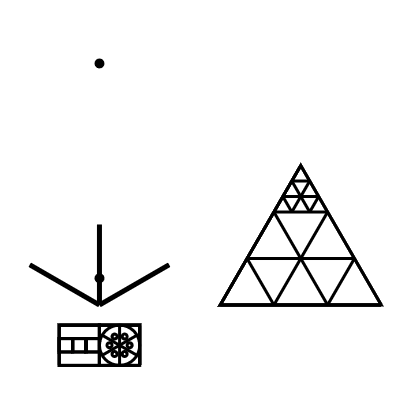
\includegraphics[width=4in]{figures/web2d/cursor3.png}
	\caption[cursor3]
	{Cursor 3.}
\end{figure}
\begin{figure}
	\centering
	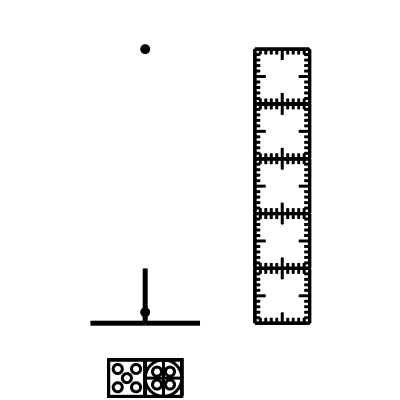
\includegraphics[width=4in]{figures/web2d/cursor5.png}
	\caption[cursor5]
	{Cursor 5.}
\end{figure}





\begin{itemize}
\tightlist
\item
hello world vesica piscis
\item
symbols, how they work with hypercube, 
\item
editing, cursor, keyboards, control panels, modes
\item
symmetries and scales, different methods of geometron(AG)
\item
cursor,movements, basic constructions(segment, circle, arc, dot)
\item
layers, colors, lines, style json, working with styles, transparency in hex colors, finding colors
\item
bezier curves
\item
paths
\item
character stack
\item
fonts
\item
flags
\item
tracing symbols from images
\item
editing the hypercube and shape table, sharing them, import and export of hypercube, sharing of bytecode
\item
canvas,svg/png/base64 workflow, laser cut shapes production, practical graphics for manuscripts and web, iconsymbols, usage in jupyter notebooks, how the JSON embeds in the SVG, how the symbol feed works, how the setup of JSON works,
\item
control panels, softkey interfaces, writing geometron apps, how to replicate in other systems from scratch
\item
examples of using the GVM in JS, documentation of geometron.js, how to use just as a js library to build whatever you want, a list of things someone needs to build to make all this a lot better, how to do that
\end{itemize}